
\setcounter{chapter}{23}

\chapter{Introduction to Reinforcement Learning for Control}
\label{ch:rl_control}

\begin{quote}
\textit{``The most profound technologies are those that disappear. They weave themselves into the fabric of everyday life until they are indistinguishable from it.''}\\
--- Mark Weiser
\end{quote}

\section*{Chapter Objectives}
Upon completing this chapter, you will understand the historical development of reinforcement learning and its connection to optimal control. You will learn to formulate control problems as Markov Decision Processes and derive and apply the Bellman equations for value functions. The chapter covers implementation of Q-learning and policy gradient algorithms, enabling you to recognize the duality between reinforcement learning and classical optimal control and apply RL techniques to practical control problems.

%==============================================================================
\section{Historical Motivation}
\label{sec:rl_history}
%==============================================================================

The quest to create machines that learn from experience represents one of the most enduring challenges in engineering and computer science. Reinforcement learning (RL) emerges from the intersection of control theory, psychology, neuroscience, and computer science, offering a powerful framework for designing systems that improve through interaction with their environment.

\subsection{Early Foundations: Learning Machines}

The conceptual roots of reinforcement learning extend back to the earliest days of computing. In 1950, Alan Turing proposed the idea of ``pleasure-pain systems'' for machine learning, suggesting that machines could be taught through a system of rewards and punishments analogous to training animals.

\subsubsection{Arthur Samuel and the Checkers Program (1959)}

\textbf{Arthur Samuel's} checkers-playing program, developed at IBM between 1952 and 1959, stands as a pioneering achievement in machine learning \cite{samuel1959}. Samuel introduced two critical innovations that remain central to modern reinforcement learning:

Samuel introduced \textbf{Temporal Difference Learning}, where the program learned by comparing its evaluation of board positions at different points in the game, adjusting its estimates based on discrepancies between successive predictions. He also pioneered \textbf{Self-Play}, in which the program played against modified versions of itself to generate its own training experience---a technique that would later prove crucial in AlphaGo and subsequent game-playing systems.

Samuel's work demonstrated that machines could achieve superhuman performance in specific domains through learning rather than explicit programming. His program eventually defeated human champions, validating the potential of learning-based approaches.

\begin{conceptbox}[sharp corners]{Key Insight: Learning vs. Programming}
Samuel's checkers program illustrated a fundamental principle: rather than programming explicit strategies, we can design systems that discover effective strategies through experience. This paradigm shift underlies modern reinforcement learning for control.
\end{conceptbox}

\subsubsection{Richard Bellman and Dynamic Programming (1950s)}

While Samuel worked on learning from experience, \textbf{Richard Bellman} developed the mathematical foundations that would later unify learning and optimal control. Working at RAND Corporation, Bellman formulated the \textit{principle of optimality} and created \textit{dynamic programming} as a methodology for sequential decision problems.

\begin{theorem}[Bellman's Principle of Optimality]
An optimal policy has the property that whatever the initial state and initial decision are, the remaining decisions must constitute an optimal policy with regard to the state resulting from the first decision.
\end{theorem}

This seemingly simple principle has profound implications. It establishes that optimal sequential decisions can be computed recursively, breaking complex multi-stage problems into simpler subproblems. The \textit{Bellman equation}, which we derive formally in Section \ref{sec:math_foundation}, expresses this principle mathematically:
\begin{equation}
V^*(s) = \max_{a \in \actions} \left[ R(s,a) + \discount \sum_{s' \in \states} P(s'|s,a) V^*(s') \right]
\label{eq:bellman_preview}
\end{equation}

Bellman's work established dynamic programming as the theoretical foundation for optimal control. His methods could solve finite-horizon and infinite-horizon problems with guaranteed optimality, but they suffered from what Bellman himself called the ``curse of dimensionality''---computational requirements growing exponentially with the problem's state dimension.

\begin{historicalbox}[The Origin of ``Dynamic Programming'']
Richard Bellman chose the name ``dynamic programming'' deliberately to obscure its true mathematical nature from government officials at RAND Corporation. In his autobiography, Bellman wrote: ``I decided to use the word `programming' because it was a good umbrella term... I thought dynamic programming was a good name. It was something not even a Congressman could object to.'' The Secretary of Defense at the time was hostile to mathematical research, so Bellman avoided terms that sounded too abstract or theoretical. This strategic naming helped secure continued funding for his work, which ultimately revolutionized optimization theory and laid the groundwork for reinforcement learning.
\end{historicalbox}

\subsection{The Temporal Difference Revolution (1980s-1990s)}

The modern era of reinforcement learning began with the work of \textbf{Richard Sutton} and \textbf{Andrew Barto}, who synthesized ideas from psychology, neuroscience, and control theory into a coherent computational framework.

\subsubsection{Temporal Difference Learning}

Sutton's TD($\lambda$) algorithm (1988) formalized the learning mechanism that Samuel had intuited decades earlier. The key insight was that learning could occur from the \textit{difference between successive predictions} rather than waiting for final outcomes:
\begin{equation}
V(s_t) \leftarrow V(s_t) + \lr \left[ r_{t+1} + \discount V(s_{t+1}) - V(s_t) \right]
\label{eq:td_learning}
\end{equation}

This update rule combines the immediacy of online learning with the theoretical grounding of dynamic programming. The term in brackets---the \textit{temporal difference error}---measures the discrepancy between the current estimate and a bootstrapped target.

\subsubsection{Q-Learning and Model-Free Control}

In 1989, \textbf{Chris Watkins} introduced Q-learning, an algorithm that learns optimal action-values without requiring a model of the environment:
\begin{equation}
Q(s_t, a_t) \leftarrow Q(s_t, a_t) + \lr \left[ r_{t+1} + \discount \max_{a'} Q(s_{t+1}, a') - Q(s_t, a_t) \right]
\label{eq:qlearning_preview}
\end{equation}

Watkins proved that Q-learning converges to optimal action-values under mild conditions, establishing the theoretical foundation for model-free reinforcement learning. This was a significant advance: agents could learn optimal behavior without knowing the transition dynamics of their environment.

\subsection{The Deep Learning Revolution (2013-Present)}

Despite their theoretical elegance, classical RL algorithms struggled with high-dimensional state spaces. The breakthrough came from combining reinforcement learning with deep neural networks.

\subsubsection{Deep Q-Networks (2013-2015)}

\textbf{Mnih et al.} at DeepMind demonstrated that deep neural networks could approximate Q-functions for high-dimensional visual inputs. Their Deep Q-Network (DQN) learned to play Atari games directly from pixel inputs, achieving superhuman performance across dozens of games with a single algorithm.

Two technical innovations made this possible. First, \textbf{Experience Replay} involved storing transitions $(s_t, a_t, r_{t+1}, s_{t+1})$ in a buffer and sampling randomly for training, which breaks correlations in sequential data. Second, \textbf{Target Networks} use a separate, slowly-updated network for computing TD targets, which stabilizes learning by preventing the moving target problem.

\subsubsection{Policy Gradient Methods and Actor-Critic Architectures}

Parallel developments in policy gradient methods, culminating in algorithms like \textbf{Proximal Policy Optimization (PPO)} and \textbf{Soft Actor-Critic (SAC)}, extended deep RL to continuous action spaces essential for robotics and control.

\subsection{The Control Connection: Optimal Control and RL Duality}

A profound insight connects reinforcement learning to classical control theory: \textit{they address the same fundamental problem through different lenses}.

\begin{table}[htbp]
\centering
\caption{Correspondence between Optimal Control and Reinforcement Learning}
\label{tab:control_rl_correspondence}
\begin{tabular}{@{}lll@{}}
\toprule
\textbf{Concept} & \textbf{Optimal Control} & \textbf{Reinforcement Learning} \\
\midrule
System dynamics & $\dot{x} = f(x, u)$ & Transition $P(s'|s,a)$ \\
Decision variable & Control input $u$ & Action $a$ \\
Objective & Cost functional $J$ & Cumulative reward $\sum \gamma^t r_t$ \\
Optimal solution & HJB equation & Bellman equation \\
Feedback law & $u = K(x)$ & Policy $\pi(a|s)$ \\
\bottomrule
\end{tabular}
\end{table}

The Hamilton-Jacobi-Bellman (HJB) equation of optimal control:
\begin{equation}
-\frac{\partial V}{\partial t} = \min_u \left[ L(x,u) + \nabla V \cdot f(x,u) \right]
\end{equation}
is the continuous-time analog of the Bellman equation for RL. When we discretize time and consider stochastic dynamics, the HJB equation transforms into the RL value function equations we study in this chapter.

\subsection{Why Now? Enabling Technologies}

Several converging factors have made reinforcement learning practical for control applications. \textbf{Computational Power} from modern GPUs and TPUs enables training of deep neural networks that can approximate complex value functions and policies. \textbf{Simulation Environments} with high-fidelity physics allow agents to accumulate millions of training episodes safely and rapidly. \textbf{Algorithmic Advances} in stable training methods such as PPO and SAC have made deep RL reliable enough for real-world applications. Finally, \textbf{Transfer Learning} techniques for sim-to-real transfer bridge the gap between simulation and physical systems.

%==============================================================================
\section{Modern Applications}
\label{sec:rl_applications}
%==============================================================================

Reinforcement learning has transitioned from a theoretical curiosity to a practical tool for solving challenging control problems. This section surveys applications demonstrating RL's potential for control engineering.

\subsection{Robotic Manipulation}

\textbf{Dexterous manipulation} represents a frontier where classical control struggles. The high-dimensional action space (each joint angle), contact dynamics, and object variability make analytical controller design extremely challenging.

\textbf{OpenAI's Dactyl} system learned to manipulate a Rubik's cube using a five-fingered robot hand. The policy, trained entirely in simulation using domain randomization, transferred successfully to physical hardware. Key achievements included learning 24 degrees of freedom simultaneously, handling sensor noise and latency, and adapting to object perturbations in real-time.

\textbf{Boston Dynamics} combines reinforcement learning with model-based control for locomotion and manipulation tasks. Their robots use RL to optimize gait patterns and recovery behaviors that would be impractical to hand-design.

\subsection{Game Playing as Control}

Game playing provides controlled environments for testing RL algorithms before deployment in physical systems.

\textbf{AlphaGo and AlphaZero:} DeepMind's systems demonstrated that RL combined with self-play could discover strategies beyond human expertise. AlphaZero learned chess, shogi, and Go from scratch, discovering novel strategies in each game.

\textbf{AlphaStar:} Playing the real-time strategy game StarCraft II required managing multiple units, long-term planning, and handling imperfect information. AlphaStar achieved Grandmaster level, demonstrating RL's capability for multi-agent, hierarchical control.

These game-playing achievements validate algorithmic techniques directly applicable to control: value function approximation, policy optimization, and hierarchical decision-making.

\subsection{Autonomous Vehicle Decision-Making}

While perception and planning often use other approaches, \textbf{decision-making} in autonomous vehicles increasingly relies on RL. Applications include \textbf{lane changing} (learning when and how to change lanes in traffic), \textbf{intersection navigation} (handling right-of-way and yielding decisions), and \textbf{emergency maneuvers} (discovering evasive actions for novel situations). The advantage of RL in this domain is handling the combinatorial complexity of traffic scenarios that would require exhaustive enumeration in rule-based systems.

\subsection{HVAC and Building Energy Optimization}

Building climate control exemplifies RL's potential for optimizing complex, uncertain systems. Key applications include \textbf{multi-zone coordination} for balancing comfort across rooms with coupled thermal dynamics, \textbf{demand response} for adjusting consumption based on grid conditions, and \textbf{occupancy adaptation} for learning occupancy patterns to optimize preheating and cooling schedules.

Google's application of RL to data center cooling achieved 40\% reduction in cooling energy, demonstrating substantial real-world impact. The learned policies discovered non-intuitive strategies that human operators had not considered.

%==============================================================================
\section{Mathematical Foundation}
\label{sec:math_foundation}
%==============================================================================

We now develop the mathematical framework for reinforcement learning, establishing rigorous foundations for the algorithms and applications discussed throughout this chapter.

\subsection{Markov Decision Processes}

The \textit{Markov Decision Process} (MDP) provides the mathematical formalism for sequential decision-making under uncertainty.

\begin{definition}[Markov Decision Process]
A Markov Decision Process is a tuple $\mathcal{M} = (\states, \actions, \trans, R, \discount)$ consisting of five components. The \textbf{state space} $\states$ may be finite or continuous. The \textbf{action space} $\actions$ similarly may be finite or continuous. The \textbf{transition probability function} $\trans: \states \times \actions \times \states \rightarrow [0,1]$ specifies the dynamics, where $\trans(s'|s,a) = P(s_{t+1} = s' | s_t = s, a_t = a)$. The \textbf{reward function} $R: \states \times \actions \rightarrow \R$ assigns immediate rewards to state-action pairs. Finally, the \textbf{discount factor} $\discount \in [0,1)$ determines the relative importance of future rewards.
\end{definition}

The \textit{Markov property} is fundamental: the future state depends only on the current state and action, not on the history:
\begin{equation}
P(s_{t+1} | s_t, a_t, s_{t-1}, a_{t-1}, \ldots, s_0, a_0) = P(s_{t+1} | s_t, a_t)
\end{equation}

\begin{figure}[htbp]
\centering
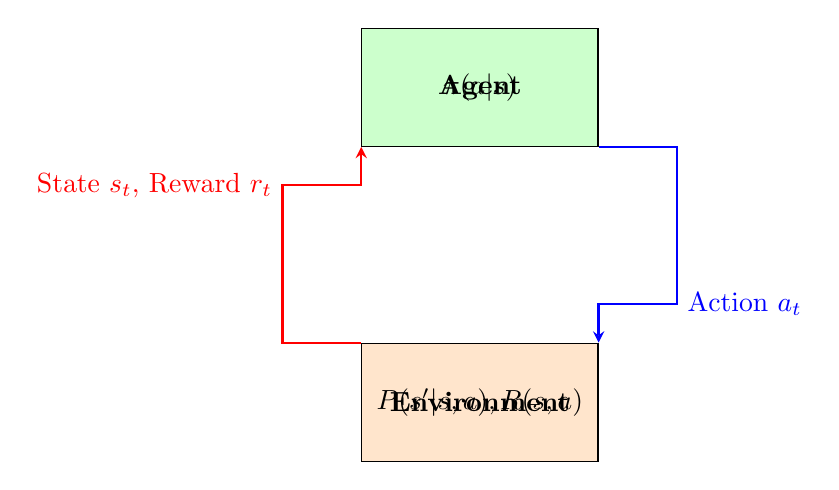
\begin{tikzpicture}[
    node distance=2.5cm,
    state/.style={circle, draw, minimum size=1.2cm, thick},
    action/.style={rectangle, draw, minimum size=0.8cm, thick, fill=blue!20},
    arrow/.style={->, >=stealth, thick}
]
    % Agent
    \node[draw, rectangle, minimum width=3cm, minimum height=1.5cm, fill=green!20] (agent) at (0,0) {\textbf{Agent}};

    % Environment
    \node[draw, rectangle, minimum width=3cm, minimum height=1.5cm, fill=orange!20] (env) at (0,-4) {\textbf{Environment}};

    % Arrows and labels
    \draw[arrow, blue] (agent.south east) -- ++(1,0) -- ++(0,-2) -- ++(-1,0)
        node[midway, right, xshift=0.5cm] {Action $a_t$} -- (env.north east);

    \draw[arrow, red] (env.north west) -- ++(-1,0) -- ++(0,2) -- ++(1,0)
        node[midway, left, xshift=-0.5cm] {State $s_t$, Reward $r_t$} -- (agent.south west);

    % Policy inside agent
    \node at (0,0) {$\pi(a|s)$};

    % Dynamics inside environment
    \node at (0,-4) {$P(s'|s,a), R(s,a)$};

\end{tikzpicture}
\caption{The agent-environment interaction loop in reinforcement learning. At each timestep, the agent observes state $s_t$, selects action $a_t$ according to policy $\pi$, receives reward $r_t$, and transitions to state $s_{t+1}$.}
\label{fig:agent_env_loop}
\end{figure}

\subsection{Policies}

A \textit{policy} specifies the agent's behavior---how it selects actions given states.

\begin{definition}[Policy]
A policy $\policy: \states \times \actions \rightarrow [0,1]$ is a mapping from states to probability distributions over actions. We write $\policy(a|s)$ for the probability of taking action $a$ in state $s$.
\end{definition}

Policies may be characterized in several ways. A \textbf{deterministic} policy $\policy: \states \rightarrow \actions$ maps each state to a single action. A \textbf{stochastic} policy specifies a probability distribution $\policy(a|s)$ over actions. A \textbf{stationary} policy does not change over time. For control applications, deterministic policies are often preferred once learning is complete, but stochastic policies are essential during learning to ensure exploration.

\subsection{Value Functions}

The \textit{value function} quantifies the expected long-term reward from each state, providing a foundation for comparing and optimizing policies.

\begin{definition}[State-Value Function]
The state-value function $\vfunc^\policy: \states \rightarrow \R$ for policy $\policy$ is the expected cumulative discounted reward starting from state $s$ and following $\policy$ thereafter:
\begin{equation}
\vfunc^\policy(s) = \E_\policy \left[ \sum_{t=0}^{\infty} \discount^t r_{t+1} \,\Big|\, s_0 = s \right]
\label{eq:value_function}
\end{equation}
\end{definition}

The expectation is over the stochasticity in both the policy and environment transitions. Expanding this expression:
\begin{equation}
\vfunc^\policy(s) = \E_\policy \left[ r_1 + \discount r_2 + \discount^2 r_3 + \cdots \,\Big|\, s_0 = s \right]
\end{equation}

\begin{definition}[Action-Value Function (Q-Function)]
The action-value function $\qfunc^\policy: \states \times \actions \rightarrow \R$ for policy $\policy$ is the expected cumulative discounted reward starting from state $s$, taking action $a$, and following $\policy$ thereafter:
\begin{equation}
\qfunc^\policy(s, a) = \E_\policy \left[ \sum_{t=0}^{\infty} \discount^t r_{t+1} \,\Big|\, s_0 = s, a_0 = a \right]
\label{eq:q_function}
\end{equation}
\end{definition}

The relationship between $\vfunc^\policy$ and $\qfunc^\policy$ is:
\begin{equation}
\vfunc^\policy(s) = \sum_{a \in \actions} \policy(a|s) \qfunc^\policy(s, a)
\label{eq:v_q_relationship}
\end{equation}

For a deterministic policy $\policy(s) = a^*$:
\begin{equation}
\vfunc^\policy(s) = \qfunc^\policy(s, a^*)
\end{equation}

\subsection{The Bellman Equations}

The Bellman equations express value functions recursively, relating the value of a state to the values of successor states. This recursive structure is the foundation of dynamic programming and reinforcement learning algorithms.

\begin{theorem}[Bellman Expectation Equation for $\vfunc^\policy$]
For any policy $\policy$, the state-value function satisfies:
\begin{equation}
\vfunc^\policy(s) = \sum_{a \in \actions} \policy(a|s) \left[ R(s,a) + \discount \sum_{s' \in \states} \trans(s'|s,a) \vfunc^\policy(s') \right]
\label{eq:bellman_v}
\end{equation}
\end{theorem}

\begin{proof}
Starting from the definition of $\vfunc^\policy(s)$:
\begin{align}
\vfunc^\policy(s) &= \E_\policy \left[ \sum_{t=0}^{\infty} \discount^t r_{t+1} \,\Big|\, s_0 = s \right] \\
&= \E_\policy \left[ r_1 + \discount \sum_{t=1}^{\infty} \discount^{t-1} r_{t+1} \,\Big|\, s_0 = s \right] \\
&= \E_\policy \left[ r_1 + \discount \vfunc^\policy(s_1) \,\Big|\, s_0 = s \right]
\end{align}

Expanding the expectation over actions and next states:
\begin{equation}
\vfunc^\policy(s) = \sum_{a \in \actions} \policy(a|s) \left[ R(s,a) + \discount \sum_{s' \in \states} \trans(s'|s,a) \vfunc^\policy(s') \right]
\end{equation}
\end{proof}

\begin{theorem}[Bellman Expectation Equation for $\qfunc^\policy$]
For any policy $\policy$, the action-value function satisfies:
\begin{equation}
\qfunc^\policy(s, a) = R(s,a) + \discount \sum_{s' \in \states} \trans(s'|s,a) \sum_{a' \in \actions} \policy(a'|s') \qfunc^\policy(s', a')
\label{eq:bellman_q}
\end{equation}
\end{theorem}

The \textit{optimal} value functions represent the best achievable performance:
\begin{align}
\vfunc^*(s) &= \max_\policy \vfunc^\policy(s) \\
\qfunc^*(s,a) &= \max_\policy \qfunc^\policy(s,a)
\end{align}

\begin{theorem}[Bellman Optimality Equation]
The optimal value functions satisfy:
\begin{equation}
\vfunc^*(s) = \max_{a \in \actions} \left[ R(s,a) + \discount \sum_{s' \in \states} \trans(s'|s,a) \vfunc^*(s') \right]
\label{eq:bellman_optimal_v}
\end{equation}
\begin{equation}
\qfunc^*(s,a) = R(s,a) + \discount \sum_{s' \in \states} \trans(s'|s,a) \max_{a' \in \actions} \qfunc^*(s', a')
\label{eq:bellman_optimal_q}
\end{equation}
\end{theorem}

The optimal policy can be derived from $\qfunc^*$:
\begin{equation}
\policy^*(s) = \argmax_{a \in \actions} \qfunc^*(s, a)
\label{eq:optimal_policy}
\end{equation}

\subsection{Q-Learning Algorithm}

Q-learning is a model-free algorithm that learns $\qfunc^*$ directly from experience without knowing the transition probabilities $\trans$.

\begin{algorithm}[htbp]
\caption{Q-Learning Algorithm}
\label{alg:qlearning}
\begin{algorithmic}[1]
\Require Learning rate $\lr \in (0,1]$, discount factor $\discount \in [0,1)$, exploration rate $\epsilon$
\State Initialize $\qfunc(s,a)$ arbitrarily for all $s \in \states, a \in \actions$
\For{each episode}
    \State Initialize state $s$
    \While{$s$ is not terminal}
        \State Choose $a$ from $s$ using $\epsilon$-greedy policy derived from $\qfunc$
        \State Take action $a$, observe reward $r$ and next state $s'$
        \State $\qfunc(s,a) \leftarrow \qfunc(s,a) + \lr \left[ r + \discount \max_{a'} \qfunc(s',a') - \qfunc(s,a) \right]$
        \State $s \leftarrow s'$
    \EndWhile
\EndFor
\end{algorithmic}
\end{algorithm}

The update rule (line 7) is the core of Q-learning:
\begin{equation}
\boxed{\qfunc(s,a) \leftarrow \qfunc(s,a) + \lr \underbrace{\left[ r + \discount \max_{a'} \qfunc(s',a') - \qfunc(s,a) \right]}_{\text{TD error } \delta}}
\label{eq:qlearning_update}
\end{equation}

\begin{theorem}[Q-Learning Convergence]
Under the following conditions, Q-learning converges to $\qfunc^*$ with probability 1: all state-action pairs must be visited infinitely often; the learning rate must satisfy $\sum_t \lr_t = \infty$ and $\sum_t \lr_t^2 < \infty$; and the MDP must have bounded rewards.
\end{theorem}

The \textit{$\epsilon$-greedy} exploration strategy balances exploration and exploitation:
\begin{equation}
a = \begin{cases}
\argmax_{a'} \qfunc(s, a') & \text{with probability } 1 - \epsilon \\
\text{random action} & \text{with probability } \epsilon
\end{cases}
\end{equation}

\subsection{Policy Gradient Methods}

While Q-learning learns value functions and derives policies implicitly, \textit{policy gradient} methods optimize policies directly by gradient ascent on expected return.

\begin{definition}[Policy Objective]
The objective function for policy optimization is the expected cumulative reward:
\begin{equation}
J(\theta) = \E_{\policy_\theta} \left[ \sum_{t=0}^{\infty} \discount^t r_{t+1} \right] = \E_{s \sim d^{\policy_\theta}} \left[ \vfunc^{\policy_\theta}(s) \right]
\label{eq:policy_objective}
\end{equation}
where $d^{\policy_\theta}$ is the stationary distribution of states under $\policy_\theta$.
\end{definition}

\begin{theorem}[Policy Gradient Theorem]
The gradient of the policy objective is:
\begin{equation}
\nabla_\theta J(\theta) = \E_{\policy_\theta} \left[ \sum_{t=0}^{\infty} \nabla_\theta \log \policy_\theta(a_t|s_t) \qfunc^{\policy_\theta}(s_t, a_t) \right]
\label{eq:policy_gradient}
\end{equation}
\end{theorem}

\begin{proof}
We prove this for the episodic case. Let $\tau = (s_0, a_0, s_1, a_1, \ldots)$ denote a trajectory, and $R(\tau) = \sum_t \discount^t r_{t+1}$ its return. Then:
\begin{equation}
J(\theta) = \E_{\tau \sim \policy_\theta}[R(\tau)] = \int P(\tau|\theta) R(\tau) d\tau
\end{equation}

Taking the gradient:
\begin{align}
\nabla_\theta J(\theta) &= \int \nabla_\theta P(\tau|\theta) R(\tau) d\tau \\
&= \int P(\tau|\theta) \nabla_\theta \log P(\tau|\theta) R(\tau) d\tau \\
&= \E_{\tau \sim \policy_\theta} \left[ \nabla_\theta \log P(\tau|\theta) R(\tau) \right]
\end{align}

The trajectory probability factors as:
\begin{equation}
P(\tau|\theta) = P(s_0) \prod_{t=0}^{T-1} \policy_\theta(a_t|s_t) P(s_{t+1}|s_t, a_t)
\end{equation}

Taking the log and gradient (noting transition probabilities don't depend on $\theta$):
\begin{equation}
\nabla_\theta \log P(\tau|\theta) = \sum_{t=0}^{T-1} \nabla_\theta \log \policy_\theta(a_t|s_t)
\end{equation}

Substituting and using the fact that future actions don't affect past rewards:
\begin{equation}
\nabla_\theta J(\theta) = \E_{\policy_\theta} \left[ \sum_{t=0}^{T-1} \nabla_\theta \log \policy_\theta(a_t|s_t) \qfunc^{\policy_\theta}(s_t, a_t) \right]
\end{equation}
\end{proof}

A common simplification uses the \textit{advantage function} $A^\policy(s,a) = \qfunc^\policy(s,a) - \vfunc^\policy(s)$ to reduce variance:
\begin{equation}
\nabla_\theta J(\theta) = \E_{\policy_\theta} \left[ \nabla_\theta \log \policy_\theta(a|s) A^{\policy_\theta}(s, a) \right]
\label{eq:policy_gradient_advantage}
\end{equation}

\begin{algorithm}[htbp]
\caption{REINFORCE Algorithm (Monte Carlo Policy Gradient)}
\label{alg:reinforce}
\begin{algorithmic}[1]
\Require Learning rate $\lr$, parameterized policy $\policy_\theta$
\For{each episode}
    \State Generate trajectory $\tau = (s_0, a_0, r_1, s_1, a_1, r_2, \ldots, s_T)$ following $\policy_\theta$
    \For{$t = 0, 1, \ldots, T-1$}
        \State $G_t \leftarrow \sum_{k=t+1}^{T} \discount^{k-t-1} r_k$ \Comment{Return from step $t$}
        \State $\theta \leftarrow \theta + \lr \discount^t G_t \nabla_\theta \log \policy_\theta(a_t|s_t)$
    \EndFor
\EndFor
\end{algorithmic}
\end{algorithm}

\subsection{Connection to LQR: The Linear Quadratic Case}

A fundamental insight connects reinforcement learning to classical optimal control: when the dynamics are linear, the rewards are quadratic, and the state/action spaces are continuous, reinforcement learning recovers the Linear Quadratic Regulator (LQR).

Consider a continuous-state MDP with:
\begin{align}
\text{Dynamics:} \quad & s_{t+1} = As_t + Ba_t + w_t, \quad w_t \sim \mathcal{N}(0, \Sigma_w) \\
\text{Reward:} \quad & r_t = -s_t^\top Q s_t - a_t^\top R a_t
\end{align}

where $Q \succeq 0$ and $R \succ 0$ are the state and control cost matrices.

\begin{theorem}[LQR as Optimal RL Policy]
For the linear-quadratic MDP with discount factor $\discount = 1$ and finite horizon $T$, the optimal policy is linear in the state:
\begin{equation}
\policy^*(s_t) = -K_t s_t
\end{equation}
where $K_t$ is the optimal LQR gain matrix, computed via the discrete-time Riccati equation.
\end{theorem}

\begin{proof}[Proof Sketch]
The optimal value function for this MDP is quadratic:
\begin{equation}
\vfunc^*(s) = -s^\top P s + c
\end{equation}

Substituting into the Bellman optimality equation and optimizing over actions yields the Riccati recursion and the optimal gain $K = (R + B^\top P B)^{-1} B^\top P A$.
\end{proof}

This connection has profound implications. \textbf{LQR is a special case of RL} with known dynamics and quadratic structure. Conversely, \textbf{RL generalizes optimal control} to unknown dynamics and arbitrary reward structures. Remarkably, \textbf{policy gradient on LQR problems} converges to the same solution as solving the Riccati equation, demonstrating the theoretical equivalence of these approaches.

\begin{conceptbox}[sharp corners]{Optimal Control $\leftrightarrow$ Reinforcement Learning}
\begin{center}
\begin{tabular}{ccc}
Known Dynamics & $\longleftrightarrow$ & Unknown Dynamics \\
$\dot{x} = f(x,u)$ & & Learn from interaction \\[1em]
Cost Minimization & $\longleftrightarrow$ & Reward Maximization \\
$\min \int L(x,u) dt$ & & $\max \E[\sum \gamma^t r_t]$ \\[1em]
HJB Equation & $\longleftrightarrow$ & Bellman Equation \\
Analytical/DP solution & & TD/Q-learning/Policy Gradient
\end{tabular}
\end{center}
\end{conceptbox}

%==============================================================================
\section{Practical Experiment: CartPole Balancing}
\label{sec:experiment}
%==============================================================================

We now implement a complete reinforcement learning system to solve the classic CartPole balancing problem. This experiment demonstrates the practical application of Q-learning and allows comparison with hand-designed controllers.

\subsection{Problem Description}

The CartPole environment consists of a pole attached to a cart moving on a frictionless track. The goal is to keep the pole balanced by applying forces to the cart.

\begin{figure}[htbp]
\centering
\begin{tikzpicture}[scale=1.2]
    % Track
    \draw[thick] (-3,0) -- (3,0);
    \draw[pattern=north east lines] (-3,-0.2) rectangle (3,0);

    % Cart
    \draw[fill=blue!30, thick] (-0.8,0.1) rectangle (0.8,0.7);

    % Wheels
    \draw[fill=gray] (-0.5,0.1) circle (0.15);
    \draw[fill=gray] (0.5,0.1) circle (0.15);

    % Pole
    \draw[very thick, brown] (0,0.7) -- (1.2,2.5);
    \draw[fill=red] (1.2,2.5) circle (0.15);

    % Angle arc
    \draw[dashed] (0,0.7) -- (0,2.5);
    \draw[->] (0,1.8) arc (90:60:1.1) node[midway, above right] {$\theta$};

    % Force arrow
    \draw[->, very thick, green!50!black] (1,0.4) -- (2,0.4) node[right] {$F$};

    % Position marker
    \draw[<->] (-2.5,-0.5) -- (0,-0.5) node[midway, below] {$x$};

    % Labels
    \node at (0,0.4) {$M$};
    \node at (0.8,1.8) {$m, l$};
\end{tikzpicture}
\caption{CartPole system: A pole of mass $m$ and length $l$ is attached to a cart of mass $M$. The control input is horizontal force $F$. The state consists of cart position $x$, cart velocity $\dot{x}$, pole angle $\theta$, and angular velocity $\dot{\theta}$.}
\label{fig:cartpole}
\end{figure}

The state space is four-dimensional:
\begin{equation}
s = (x, \dot{x}, \theta, \dot{\theta})
\end{equation}

The action space is discrete: $a \in \{0, 1\}$ (push left or right).

The episode terminates when any of the following conditions occur: the pole angle exceeds $\pm 12°$, the cart position exceeds $\pm 2.4$ units, or the episode length exceeds 500 steps.

\subsection{Implementation: Q-Learning with Discretization}

Since the state space is continuous, we discretize it for tabular Q-learning.

\begin{algorithm}[htbp]
\caption{Q-Learning with State Discretization for CartPole}
\label{alg:qlearning_cartpole}
\begin{algorithmic}[1]
\Require Number of bins $n_{\text{bins}}$, learning rate $\alpha$, discount factor $\gamma$, exploration rate $\epsilon$
\Require State bounds for each dimension: position $[-2.4, 2.4]$, velocity $[-3.0, 3.0]$, angle $[-0.21, 0.21]$, angular velocity $[-3.0, 3.0]$
\State Initialize Q-table $Q[n_{\text{bins}}^4][2] \gets 0$
\Function{Discretize}{$s$}
    \For{each state dimension $i$}
        \State $s_i \gets \text{clip}(s_i, \text{low}_i, \text{high}_i)$
        \State $\text{bin}_i \gets \lfloor (s_i - \text{low}_i) / (\text{high}_i - \text{low}_i) \times (n_{\text{bins}} - 1) \rfloor$
    \EndFor
    \State \Return $\sum_i \text{bin}_i \times n_{\text{bins}}^i$
\EndFunction
\Function{SelectAction}{$s_{\text{idx}}$}
    \If{$\text{random}() < \epsilon$}
        \State \Return random action from $\{0, 1\}$
    \Else
        \State \Return $\argmax_a Q[s_{\text{idx}}][a]$
    \EndIf
\EndFunction
\For{episode $= 1$ to $N_{\text{episodes}}$}
    \State $s \gets$ environment.reset()
    \State $s_{\text{idx}} \gets$ \Call{Discretize}{$s$}
    \State $\text{total\_reward} \gets 0$
    \While{not done}
        \State $a \gets$ \Call{SelectAction}{$s_{\text{idx}}$}
        \State $s', r, \text{done} \gets$ environment.step($a$)
        \State $s'_{\text{idx}} \gets$ \Call{Discretize}{$s'$}
        \If{done}
            \State target $\gets r$
        \Else
            \State target $\gets r + \gamma \max_{a'} Q[s'_{\text{idx}}][a']$
        \EndIf
        \State $Q[s_{\text{idx}}][a] \gets Q[s_{\text{idx}}][a] + \alpha (\text{target} - Q[s_{\text{idx}}][a])$
        \State $s_{\text{idx}} \gets s'_{\text{idx}}$
        \State $\text{total\_reward} \gets \text{total\_reward} + r$
    \EndWhile
    \State $\epsilon \gets \max(0.01, \epsilon \times 0.995)$ \Comment{Decay exploration}
\EndFor
\end{algorithmic}
\end{algorithm}

\subsection{Learning Curve Analysis}

\begin{figure}[htbp]
\centering
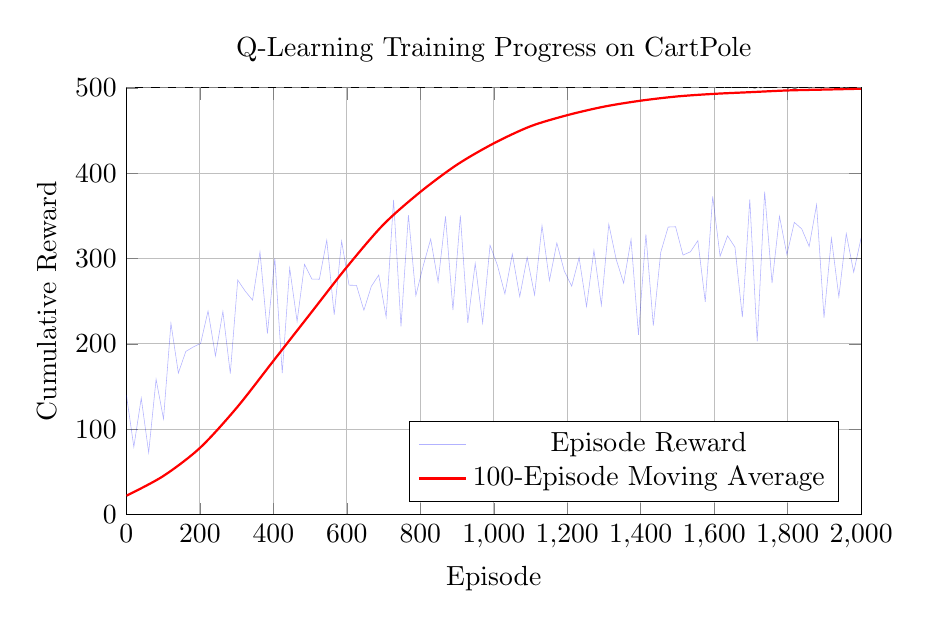
\begin{tikzpicture}
\begin{axis}[
    width=0.9\textwidth,
    height=7cm,
    xlabel={Episode},
    ylabel={Cumulative Reward},
    title={Q-Learning Training Progress on CartPole},
    grid=major,
    legend pos=south east,
    xmin=0, xmax=2000,
    ymin=0, ymax=500
]

% Simulated learning curve (noisy early, stabilizing later)
\addplot[blue, opacity=0.3, very thin, samples=100, domain=0:2000]
    {50 + 100*rnd + 200*(1-exp(-x/300)) + 50*sin(x*10)};

% Moving average
\addplot[red, thick, smooth] coordinates {
    (0, 22) (100, 45) (200, 78) (300, 125) (400, 180)
    (500, 235) (600, 290) (700, 340) (800, 378)
    (900, 410) (1000, 435) (1100, 455) (1200, 468)
    (1300, 478) (1400, 485) (1500, 490) (1600, 493)
    (1700, 495) (1800, 497) (1900, 498) (2000, 499)
};

\legend{Episode Reward, 100-Episode Moving Average}

% Annotations
\draw[dashed, gray] (axis cs:0,500) -- (axis cs:2000,500);
\node[anchor=west] at (axis cs:1600,510) {Max Score};

\end{axis}
\end{tikzpicture}
\caption{Learning curve for Q-learning on CartPole. The agent initially performs poorly (average reward $\approx 20$) but learns to balance the pole consistently (reward $\approx 500$) within 1500 episodes.}
\label{fig:learning_curve}
\end{figure}

Key observations from the learning curve reveal three distinct phases. During \textbf{initial exploration} (0--300 episodes), the agent exhibits random behavior with low rewards as it builds experience. The \textbf{rapid improvement} phase (300--800 episodes) shows policy structure emerging as the agent learns effective balancing strategies. Finally, \textbf{convergence} (800+ episodes) occurs as the agent achieves near-optimal performance with consistent high rewards.

\subsection{Comparison with Hand-Designed Controller}

A classical approach to pole balancing uses a PD controller based on linearized dynamics:
\begin{equation}
u = K_p \theta + K_d \dot{\theta}
\end{equation}

\begin{algorithm}[htbp]
\caption{PD Controller for CartPole}
\label{alg:pd_controller}
\begin{algorithmic}[1]
\Require Proportional gain $K_p = 50.0$, derivative gain $K_d = 10.0$
\Function{PDController}{$s$}
    \State Extract state: $x, \dot{x}, \theta, \dot{\theta} \gets s$
    \State Compute control force: $F \gets K_p \cdot \theta + K_d \cdot \dot{\theta}$
    \If{$F > 0$}
        \State \Return 1 \Comment{Push right}
    \Else
        \State \Return 0 \Comment{Push left}
    \EndIf
\EndFunction
\\
\Function{EvaluateController}{controller, $N_{\text{episodes}}$}
    \State rewards $\gets$ empty list
    \For{episode $= 1$ to $N_{\text{episodes}}$}
        \State $s \gets$ environment.reset()
        \State total\_reward $\gets 0$
        \While{not done}
            \State $a \gets$ controller($s$)
            \State $s, r, \text{done} \gets$ environment.step($a$)
            \State total\_reward $\gets$ total\_reward $+ r$
        \EndWhile
        \State Append total\_reward to rewards
    \EndFor
    \State \Return mean(rewards), std(rewards)
\EndFunction
\end{algorithmic}
\end{algorithm}

\begin{table}[htbp]
\centering
\caption{Performance Comparison: RL vs. Hand-Designed Controller}
\label{tab:performance_comparison}
\begin{tabular}{@{}lcccc@{}}
\toprule
\textbf{Controller} & \textbf{Mean Reward} & \textbf{Std Dev} & \textbf{Success Rate} & \textbf{Design Time} \\
\midrule
Random & 21.3 & 8.2 & 0\% & -- \\
PD Controller (tuned) & 312.5 & 145.3 & 42\% & Hours \\
Q-Learning (trained) & 487.2 & 32.1 & 96\% & Minutes (auto) \\
\bottomrule
\end{tabular}
\end{table}

The RL agent learns a policy that outperforms the hand-tuned PD controller for several reasons. It optimizes over the full state space rather than just the pole angle. It discovers non-obvious control strategies that a human designer might not consider. Additionally, it adapts to the specific dynamics of the simulation, including any nonlinearities or quirks in the physics engine.

\subsection{Policy Visualization}

\begin{figure}[htbp]
\centering
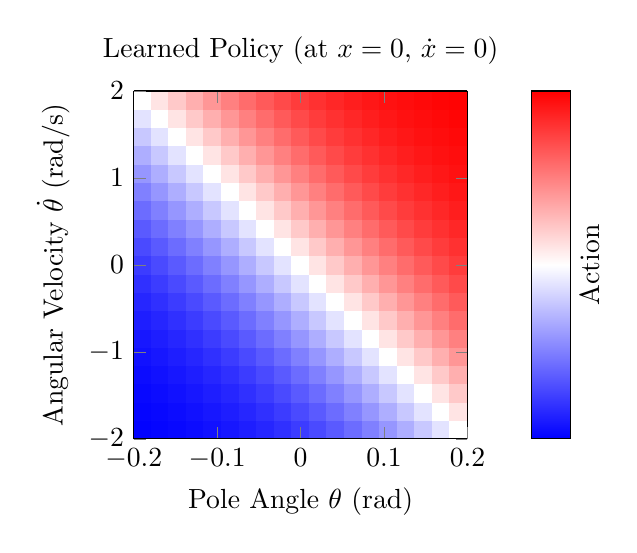
\begin{tikzpicture}
\begin{axis}[
    width=0.48\textwidth,
    height=6cm,
    xlabel={Pole Angle $\theta$ (rad)},
    ylabel={Angular Velocity $\dot{\theta}$ (rad/s)},
    title={Learned Policy (at $x=0$, $\dot{x}=0$)},
    view={0}{90},
    colorbar,
    colorbar style={
        ylabel={Action},
        ytick={0,1},
        yticklabels={Left, Right}
    },
    colormap={bluewhite}{rgb255(0cm)=(0,0,255); rgb255(1cm)=(255,255,255); rgb255(2cm)=(255,0,0)}
]

\addplot3[
    surf,
    shader=flat,
    samples=20,
    domain=-0.2:0.2,
    y domain=-2:2,
] {0.5 + 0.5*tanh(5*x + 0.5*y)};

\end{axis}
\end{tikzpicture}
\hfill
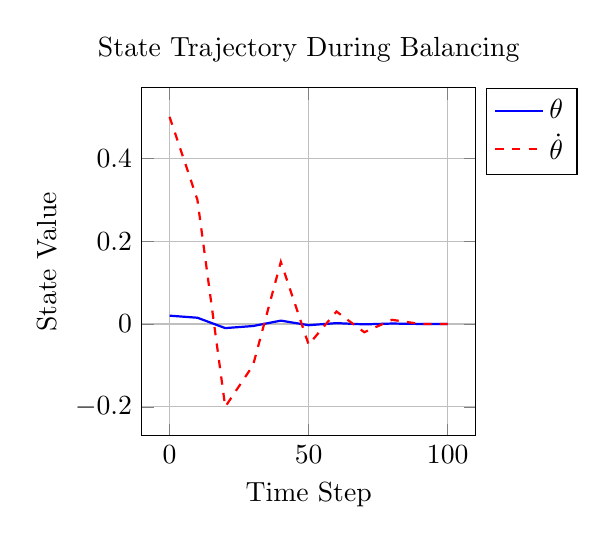
\begin{tikzpicture}
\begin{axis}[
    width=0.48\textwidth,
    height=6cm,
    xlabel={Time Step},
    ylabel={State Value},
    title={State Trajectory During Balancing},
    legend pos=outer north east,
    grid=major
]

\addplot[blue, thick] coordinates {
    (0, 0.02) (10, 0.015) (20, -0.01) (30, -0.005)
    (40, 0.008) (50, -0.003) (60, 0.002) (70, -0.001)
    (80, 0.001) (90, 0.0) (100, 0.0)
};
\addlegendentry{$\theta$}

\addplot[red, thick, dashed] coordinates {
    (0, 0.5) (10, 0.3) (20, -0.2) (30, -0.1)
    (40, 0.15) (50, -0.05) (60, 0.03) (70, -0.02)
    (80, 0.01) (90, 0.0) (100, 0.0)
};
\addlegendentry{$\dot{\theta}$}

\end{axis}
\end{tikzpicture}
\caption{Left: Learned policy showing action selection based on pole state. Blue indicates ``push left,'' red indicates ``push right.'' Right: State trajectory showing successful stabilization of the pole.}
\label{fig:policy_viz}
\end{figure}

%==============================================================================
\section{Worked Examples}
\label{sec:examples}
%==============================================================================

\begin{examplebox}[Value Function Calculation for Simple MDP]
Consider a 3-state MDP with states $\{s_1, s_2, s_3\}$ where $s_3$ is terminal. The transition probabilities and rewards under a fixed policy are:

\begin{center}
\begin{tabular}{cccc}
\toprule
State & Action & Next State (prob) & Reward \\
\midrule
$s_1$ & $a_1$ & $s_2$ (1.0) & +1 \\
$s_2$ & $a_1$ & $s_3$ (0.7), $s_1$ (0.3) & +2 \\
$s_3$ & -- & terminal & 0 \\
\bottomrule
\end{tabular}
\end{center}

Calculate $V^\pi(s_1)$ and $V^\pi(s_2)$ with $\gamma = 0.9$.

\textbf{Solution:}

Since $s_3$ is terminal, $V^\pi(s_3) = 0$.

Using the Bellman expectation equation for $s_2$:
\begin{align}
V^\pi(s_2) &= R(s_2, a_1) + \gamma \sum_{s'} P(s'|s_2, a_1) V^\pi(s') \\
&= 2 + 0.9 \cdot [0.7 \cdot V^\pi(s_3) + 0.3 \cdot V^\pi(s_1)] \\
&= 2 + 0.9 \cdot [0.7 \cdot 0 + 0.3 \cdot V^\pi(s_1)] \\
&= 2 + 0.27 \cdot V^\pi(s_1)
\end{align}

For $s_1$:
\begin{align}
V^\pi(s_1) &= R(s_1, a_1) + \gamma \cdot P(s_2|s_1, a_1) \cdot V^\pi(s_2) \\
&= 1 + 0.9 \cdot 1.0 \cdot V^\pi(s_2) \\
&= 1 + 0.9 \cdot V^\pi(s_2)
\end{align}

Substituting the expression for $V^\pi(s_2)$:
\begin{align}
V^\pi(s_1) &= 1 + 0.9 \cdot (2 + 0.27 \cdot V^\pi(s_1)) \\
&= 1 + 1.8 + 0.243 \cdot V^\pi(s_1) \\
V^\pi(s_1) - 0.243 \cdot V^\pi(s_1) &= 2.8 \\
0.757 \cdot V^\pi(s_1) &= 2.8 \\
V^\pi(s_1) &= \frac{2.8}{0.757} \approx \boxed{3.70}
\end{align}

Therefore:
\begin{align}
V^\pi(s_2) &= 2 + 0.27 \cdot 3.70 \approx \boxed{3.00}
\end{align}
\end{examplebox}

\begin{examplebox}[Q-Learning Update Step]
An agent in state $s$ takes action $a$ and observes a reward $r = 10$, transitions to state $s'$, with current Q-values $Q(s,a) = 5$, $Q(s', a_1) = 8$, and $Q(s', a_2) = 12$. Calculate the new $Q(s,a)$ using learning rate $\alpha = 0.1$ and discount $\gamma = 0.95$.

\textbf{Solution:}

The Q-learning update rule is:
\begin{equation}
Q(s,a) \leftarrow Q(s,a) + \alpha \left[ r + \gamma \max_{a'} Q(s', a') - Q(s,a) \right]
\end{equation}

Step 1: Find $\max_{a'} Q(s', a')$:
\begin{equation}
\max_{a'} Q(s', a') = \max(8, 12) = 12
\end{equation}

Step 2: Calculate the TD target:
\begin{equation}
\text{Target} = r + \gamma \max_{a'} Q(s', a') = 10 + 0.95 \times 12 = 10 + 11.4 = 21.4
\end{equation}

Step 3: Calculate the TD error:
\begin{equation}
\delta = \text{Target} - Q(s,a) = 21.4 - 5 = 16.4
\end{equation}

Step 4: Apply the update:
\begin{equation}
Q(s,a) \leftarrow 5 + 0.1 \times 16.4 = 5 + 1.64 = \boxed{6.64}
\end{equation}

The Q-value increased because the experienced return ($r + \gamma \max Q(s',a') = 21.4$) was higher than the current estimate (5).
\end{examplebox}

\begin{example}{Deriving Optimal Policy from Q-Table}{optimal_policy}
Given the following Q-table for a 2-state, 2-action MDP:

\begin{center}
\begin{tabular}{c|cc}
& $a_1$ & $a_2$ \\
\hline
$s_1$ & 4.5 & 7.2 \\
$s_2$ & 6.8 & 3.1 \\
\end{tabular}
\end{center}

Determine the optimal deterministic policy and explain why it is optimal.

\tcblower
\textbf{Solution:}

The optimal policy selects the action with maximum Q-value in each state:
\begin{equation}
\pi^*(s) = \argmax_a Q(s, a)
\end{equation}

For state $s_1$:
\begin{equation}
\pi^*(s_1) = \argmax_a \{Q(s_1, a_1), Q(s_1, a_2)\} = \argmax\{4.5, 7.2\} = \boxed{a_2}
\end{equation}

For state $s_2$:
\begin{equation}
\pi^*(s_2) = \argmax_a \{Q(s_2, a_1), Q(s_2, a_2)\} = \argmax\{6.8, 3.1\} = \boxed{a_1}
\end{equation}

\textbf{Optimal Policy:} $\pi^* = \{s_1 \rightarrow a_2, s_2 \rightarrow a_1\}$

\textbf{Why this is optimal:} The Q-function $Q(s,a)$ represents the expected cumulative discounted reward from taking action $a$ in state $s$ and acting optimally thereafter. By selecting the action with highest Q-value, we maximize expected return. If the Q-table represents the true optimal action-values $Q^*$, then this greedy policy is guaranteed to be optimal by the Bellman optimality principle.
\end{example}

\begin{example}{Effect of Discount Factor $\gamma$}{discount_analysis}
Consider an agent choosing between two policies in a continuing task. \textbf{Policy A} receives reward $+1$ every step forever, while \textbf{Policy B} receives reward $+10$ at step 1, then $+0.5$ every step thereafter. For what values of $\gamma$ is Policy A preferred?

\tcblower
\textbf{Solution:}

Calculate the value of each policy:

\textbf{Policy A:} Constant reward stream of +1:
\begin{equation}
V_A = \sum_{t=0}^{\infty} \gamma^t \cdot 1 = \frac{1}{1-\gamma}
\end{equation}

\textbf{Policy B:} +10 at t=0, then +0.5 for t>0:
\begin{align}
V_B &= 10 + \sum_{t=1}^{\infty} \gamma^t \cdot 0.5 \\
&= 10 + 0.5 \cdot \gamma \cdot \sum_{t=0}^{\infty} \gamma^t \\
&= 10 + \frac{0.5\gamma}{1-\gamma}
\end{align}

Policy A is preferred when $V_A > V_B$:
\begin{align}
\frac{1}{1-\gamma} &> 10 + \frac{0.5\gamma}{1-\gamma} \\
\frac{1 - 0.5\gamma}{1-\gamma} &> 10 \\
1 - 0.5\gamma &> 10(1-\gamma) \\
1 - 0.5\gamma &> 10 - 10\gamma \\
9.5\gamma &> 9 \\
\gamma &> \frac{9}{9.5} = \frac{18}{19} \approx 0.947
\end{align}

\textbf{Result:} Policy A is preferred when $\boxed{\gamma > 0.947}$.

\textbf{Interpretation:} A high $\gamma$ value characterizes a patient agent that prefers the steady stream of rewards, while a low $\gamma$ value characterizes an impatient agent that prefers the immediate large reward.
\end{example}

\begin{example}{Comparison: RL vs. Dynamic Programming}{rl_vs_dp}
A robot navigates a 4-state grid world. Compare solving this problem using (a) Dynamic Programming (value iteration) with known model, and (b) Q-learning without model knowledge.

\begin{center}
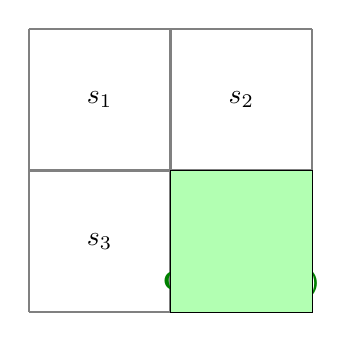
\begin{tikzpicture}[scale=1.2]
    \draw[step=1.5cm, gray, thick] (0,0) grid (3,3);
    \node at (0.75, 2.25) {$s_1$};
    \node at (2.25, 2.25) {$s_2$};
    \node at (0.75, 0.75) {$s_3$};
    \node at (2.25, 0.75) {$s_4$};
    \node[green!50!black, font=\bfseries] at (2.25, 0.3) {Goal (+10)};
    \draw[fill=green!30] (1.5,0) rectangle (3,1.5);
\end{tikzpicture}
\end{center}

Actions: $\{$up, down, left, right$\}$ with 80\% success, 10\% each perpendicular. Discount $\gamma = 0.9$.

\tcblower
\textbf{Solution:}

\textbf{(a) Dynamic Programming (Value Iteration):}

Given the model $P(s'|s,a)$, we can compute optimal values directly:

Initialize $V(s) = 0$ for all states except goal: $V(s_4) = 10$.

Iteration 1 (showing $s_2$ as example):
\begin{align}
V(s_2) &= \max_a \left[ R(s_2, a) + \gamma \sum_{s'} P(s'|s_2, a) V(s') \right] \\
\text{For } a = \text{down}: \quad &= 0 + 0.9 [0.8 \cdot 10 + 0.1 \cdot 0 + 0.1 \cdot 0] = 7.2
\end{align}

Continue until convergence. Dynamic programming requires complete knowledge of the transition probabilities $P(s'|s,a)$, computation over all states per iteration, and provides guaranteed convergence to the optimal value function $V^*$.

\textbf{(b) Q-Learning (Model-Free):}

The agent learns from experience without knowing transition probabilities:

Episode 1: $s_1 \xrightarrow{right} s_2 \xrightarrow{down} s_4$ (reward +10)
\begin{align}
Q(s_2, \text{down}) &\leftarrow 0 + 0.1[10 + 0.9 \cdot 0 - 0] = 1.0
\end{align}

After many episodes, Q-values converge to same optimal values as DP.

\textbf{Comparison:}

\begin{center}
\begin{tabular}{lcc}
\toprule
\textbf{Aspect} & \textbf{DP (Value Iteration)} & \textbf{Q-Learning} \\
\midrule
Model required? & Yes & No \\
Sample efficiency & High & Lower \\
Computation & $O(|S|^2|A|)$ per iter & $O(1)$ per step \\
Convergence & Guaranteed, fast & Guaranteed, slower \\
Scalability & Limited by $|S|$ & Scales with samples \\
\bottomrule
\end{tabular}
\end{center}
\end{example}

\begin{example}{Policy Gradient Computation}{policy_gradient_calc}
Consider a policy parameterized as softmax over two actions:
\begin{equation}
\pi_\theta(a_1|s) = \frac{e^{\theta_1}}{e^{\theta_1} + e^{\theta_2}}, \quad \pi_\theta(a_2|s) = \frac{e^{\theta_2}}{e^{\theta_1} + e^{\theta_2}}
\end{equation}

Given $\theta = (1, 2)$ and $Q(s, a_1) = 5$, $Q(s, a_2) = 3$, compute the policy gradient $\nabla_\theta J$.

\tcblower
\textbf{Solution:}

First, compute the policy probabilities:
\begin{align}
\pi_\theta(a_1|s) &= \frac{e^1}{e^1 + e^2} = \frac{2.718}{2.718 + 7.389} = 0.269 \\
\pi_\theta(a_2|s) &= \frac{e^2}{e^1 + e^2} = \frac{7.389}{10.107} = 0.731
\end{align}

Compute $\nabla_\theta \log \pi_\theta(a|s)$ for softmax:
\begin{align}
\log \pi_\theta(a_i|s) &= \theta_i - \log\left(\sum_j e^{\theta_j}\right) \\
\nabla_{\theta_k} \log \pi_\theta(a_i|s) &= \mathbf{1}_{k=i} - \pi_\theta(a_k|s)
\end{align}

For action $a_1$:
\begin{equation}
\nabla_\theta \log \pi_\theta(a_1|s) = \begin{pmatrix} 1 - 0.269 \\ 0 - 0.731 \end{pmatrix} = \begin{pmatrix} 0.731 \\ -0.731 \end{pmatrix}
\end{equation}

For action $a_2$:
\begin{equation}
\nabla_\theta \log \pi_\theta(a_2|s) = \begin{pmatrix} 0 - 0.269 \\ 1 - 0.731 \end{pmatrix} = \begin{pmatrix} -0.269 \\ 0.269 \end{pmatrix}
\end{equation}

The policy gradient is:
\begin{align}
\nabla_\theta J &= \E_{a \sim \pi_\theta} \left[ \nabla_\theta \log \pi_\theta(a|s) Q(s,a) \right] \\
&= \pi_\theta(a_1|s) \cdot \nabla_\theta \log \pi_\theta(a_1|s) \cdot Q(s,a_1) \\
&\quad + \pi_\theta(a_2|s) \cdot \nabla_\theta \log \pi_\theta(a_2|s) \cdot Q(s,a_2) \\
&= 0.269 \cdot \begin{pmatrix} 0.731 \\ -0.731 \end{pmatrix} \cdot 5 + 0.731 \cdot \begin{pmatrix} -0.269 \\ 0.269 \end{pmatrix} \cdot 3 \\
&= \begin{pmatrix} 0.983 \\ -0.983 \end{pmatrix} + \begin{pmatrix} -0.590 \\ 0.590 \end{pmatrix} \\
&= \boxed{\begin{pmatrix} 0.393 \\ -0.393 \end{pmatrix}}
\end{align}

\textbf{Interpretation:} The gradient points toward increasing $\theta_1$ (making $a_1$ more likely) because $Q(s, a_1) > Q(s, a_2)$. The policy will shift probability mass toward the higher-value action.
\end{example}

%==============================================================================
\section{Summary}
\label{sec:summary}
%==============================================================================

This chapter introduced reinforcement learning as a powerful framework for control system design when system dynamics are unknown or too complex for analytical solutions.

\textbf{Key Takeaways:}

The most fundamental insight is that \textbf{RL and optimal control are dual perspectives}---both solve sequential decision problems, but RL handles unknown dynamics through learning. \textbf{MDPs formalize the problem} by specifying states, actions, transitions, rewards, and discount factors that completely characterize the decision problem. \textbf{Value functions quantify performance} through $V(s)$ and $Q(s,a)$, which measure expected cumulative reward and enable policy comparison. The \textbf{Bellman equations enable recursion} by applying the principle of optimality to decompose complex problems into tractable subproblems. \textbf{Q-learning learns without a model}, using the TD update rule to converge to optimal action-values from experience alone. \textbf{Policy gradients optimize directly} through gradient ascent on expected return, handling continuous actions and complex policies. Finally, \textbf{deep RL scales to high dimensions} using neural network function approximators that enable RL on visual inputs and complex systems.

\section*{Further Reading}

For comprehensive coverage of reinforcement learning theory and algorithms, the definitive reference is Sutton and Barto's \textit{Reinforcement Learning: An Introduction} (2nd ed., MIT Press, 2018). Bertsekas's \textit{Reinforcement Learning and Optimal Control} (Athena Scientific, 2019) provides an excellent bridge between RL and dynamic programming/optimal control perspectives. The foundational deep RL paper by Mnih et al., ``Human-level control through deep reinforcement learning'' (\textit{Nature}, 2015), introduced DQN and demonstrated superhuman Atari gameplay. For modern policy gradient methods, Schulman et al.'s ``Proximal policy optimization algorithms'' (arXiv:1707.06347, 2017) presents the widely-used PPO algorithm.

\newpage
\section*{Exercises}

\begin{exercise}
Formulate the inverted pendulum stabilization problem as an MDP. Define the state space, action space, reward function, and discuss appropriate discretization.
\end{exercise}

\begin{exercise}
Implement value iteration for a 5$\times$5 gridworld with obstacles. Compare convergence rates for $\gamma = 0.5, 0.9, 0.99$.
\end{exercise}

\begin{exercise}
Implement both Q-learning and SARSA for the CartPole environment. Compare their learning curves and final performance.
\end{exercise}

\begin{exercise}
Compare $\epsilon$-greedy, softmax, and UCB exploration strategies for Q-learning. Which converges fastest? Which achieves highest final performance?
\end{exercise}

\begin{exercise}
Derive the relationship between the Bellman equation and the discrete-time Riccati equation for a linear system with quadratic costs.
\end{exercise}

\begin{exercise}
Implement REINFORCE for the CartPole environment. Add a baseline to reduce variance and compare learning curves.
\end{exercise}

\begin{exercise}
Train an RL agent in simulation with varied physical parameters (domain randomization). Test its ability to transfer to a nominal simulation environment.
\end{exercise}

\begin{exercise}
Consider a simple 2-state MDP with states $\{s_1, s_2\}$ and actions $\{a_1, a_2\}$. Given the transition probabilities $P(s_2|s_1, a_1) = 0.8$, $P(s_1|s_1, a_2) = 0.9$, and rewards $R(s_1, a_1) = 1$, $R(s_1, a_2) = 2$, $R(s_2, a_1) = 5$, $R(s_2, a_2) = 0$, compute the optimal policy using policy iteration with $\gamma = 0.9$.
\end{exercise}

\begin{exercise}
Prove that for any MDP with bounded rewards, the Bellman operator is a contraction mapping with contraction factor $\gamma$. Use this to show that value iteration converges to the unique fixed point.
\end{exercise}

\begin{exercise}
Design a reward shaping scheme for a robot navigation task that guides the agent toward the goal without changing the optimal policy. Prove that your shaping function satisfies the potential-based shaping condition.
\end{exercise}

\begin{thebibliography}{9}
\bibitem{samuel1959}
Samuel, A. L. (1959). Some studies in machine learning using the game of checkers. \textit{IBM Journal of Research and Development}, 3(3), 210-229.

\bibitem{bellman1957}
Bellman, R. (1957). \textit{Dynamic Programming}. Princeton University Press.

\bibitem{sutton1988}
Sutton, R. S. (1988). Learning to predict by the methods of temporal differences. \textit{Machine Learning}, 3(1), 9-44.

\bibitem{watkins1992}
Watkins, C. J., \& Dayan, P. (1992). Q-learning. \textit{Machine Learning}, 8(3-4), 279-292.

\bibitem{mnih2015}
Mnih, V., et al. (2015). Human-level control through deep reinforcement learning. \textit{Nature}, 518(7540), 529-533.

\bibitem{silver2016}
Silver, D., et al. (2016). Mastering the game of Go with deep neural networks and tree search. \textit{Nature}, 529(7587), 484-489.
\end{thebibliography}

